

\chapter{Introduction}

\label{chapterlabel2}

\section*{Chapter summary} 

In this chapter I will introduce my research. Starting with the motivation and the key concepts involved I will lead to the main research question and the subsequent question that will assist to answer the main research question. Further an outline of the dissertation will be conducted. This chapter then concludes with the overall contribution the reader can expect from reading this dissertation.\newpage


%%%%%%%%%%%%%%%%%%%%%%

\section{Motivation}

%%%%%%%%%%%%%%%%%%%%%%

\begin{figure}[!b] 
\centering
\includegraphics[height=5cm]{Illustrations/Spectacolor_JennyHolzer_.jpg}
\includegraphics[height=5cm]{Illustrations/TimesSquare.jpg}
\caption [New York Times Square in 20XX] {In 1982 media artist Jenny Holzer \index{Jenny Holzer (1950- )} explored electronic signs beyond commercial application, which led to the usage of the \textit{Spectacolor Board}. Holzer particularly choose the One Times Square's electronic display due to the orientation towards the Broadway \cite{Tate_1988} (pp.180-4). The present New York Times Square at night entirely cladded with electronic surfaces turns into a mediascape. (In the central background One Times Square building).}
\label{TimesSquare}
\end{figure}

%%%%%%%%%%%%%%%%%%%%%%
A commonly observed phenomenon of our time lets people stare at tiny mobile displays in their hands whilst neglecting their surrounding. Occasionally they bump into lamp posts but mostly it seems that ever more individual digital technologies disconnect people from physical places and people within \cite{Turkle_2012}. One may ask instead how novel digital technologies can actually support and mediate social interactions in our cities?    
In this dissertation I will argue that the integration of digital media technologies into architectural design can enhance the urban experience and eventually brings people together. 

Little is known about the effect recent digital technologies actually have on social interactions in public space and particularly on our notion of architecture. 
%Human behaviour is increasingly structured amongst others through information displays and ubiquitous mobile devices characterise our everyday culture.
Currently cities and their inhabitants are familiarising themselves with the socio-technological developments of the emerging digital age \cite{Hemment_2013}. 
Simultaneously, computer technologies increasingly affect the built environment in the way that buildings turn into computer interfaces \cite{Mitchell_1995}.
Architecture is adjusting to the requirements of novel information and communication technologies (ICTs) such as large electronic surfaces attached to building facades. For instance, the flashy New York Times Square (Fig.\ref{TimesSquare}) is an obvious example of where digital media technology has been materialised in architectural form. 

In this dissertation I consider large electronic surfaces in public spaces, referred to as \textit{Urban Screens}, \textit{Media Facades} or \textit{Media Architecture}, and their potential for mediating social interactions. More specifically I investigate the design aspects and socio-spatial settings in which temporary media architectural installations are embedded. 

The monochromic \textit{Spectacolor Board} \index{Spectacolor Board} at the New York Times building, set up in 1976, is considered to be the first large electronic surface in urban space (i.e. \textit{Urban Screen}), which broadcasts dynamic content (Fig.\ref{TimesSquare}(left)) \footnote{Knowing well that there has been the Motogram/Zipper before (link to the section where I will give more details)}. 
From then on, the prevalence of electronic surfaces in different sizes and types was unstoppable; in particular, technological developments have accelerated this trend in recent years. 
Electronic surfaces became a material to support architectural concepts and design. One of the early examples of what one may describe as \textit{Media Architecture} is Toyo Ito's \textit{Tower of Winds} \index{Tower of Winds (1986)} in Yokohama 1986 (Fig.\ref{Towerofwinds}).  More recently price decline allowed non-commercial initiatives in media art \footnote{In the field of media art the EU funded \textit{Connecting Cities Network} (CCN) \index{Connecting Cities Network (CNN)} established in between 2007-2013 an ecology of electronic surfaces that connects various media test beds and their owners around the globe with enthusiastic media technologists and artists.}, research and community engagement \footnote{In academia the \textit{Screens in the Wild} \index{Screens in the Wild (2011)} research project (in between 2011-2014), conducted at The Bartlett School of Architecture (UCL), deployed several digital and networked surfaces across communities to enhance real world connections.} to employ electronic displays for their purposes. 
One can say that media art is spearheading the exploration into interactive electronic surfaces that eventually may evoke new social practices, whilst research is uncovering new behaviours and systematically evaluates and reflects on novel phenomena.
Bringing together the domains of architecture, media art and interaction design may help architects, designers and stakeholders to better understand how to go about designing for interactions with interactive media architecture. 
Yet, part of the challenge is that there is currently only a handful of those collaborations in existence, and so there is much to learn from each attempt that unfolds a novel interactive media architecture. 


%%%%%%%%%%%%%%%%%%%%%%%

\begin{figure}[!t] 
\centering
\includegraphics[width=\textwidth]{Illustrations/Ito_T_WindTower_c_El_Croquis_1986.jpg}
\caption[\textit{Tower of Winds} by Toyo Ito, 1986, Image taken from El Croquis]{Toyo Ito's \textit{Tower of Winds} consists of a aluminium structure equipped with 12 rings consisting of 1300 multicoloured lamps, which  illuminate the old water tower. The colours dynamically change according to the wind speed that hits the tower.}
\label{Towerofwinds}
\end{figure}

%%%%%%%%%%%%%%%%%%%%%%%

%Interaction Design can be defined as 'designing interactive products to support the way people communicate and interact in their everyday and working lives' (\cite{Rogers_2015} p.8). 
An important element when designing for interactions are so called interaction spaces, which appear in the vicinity of media architectural installations. They are defined both by the characteristics of the architectural layout and the space in which they are situated, along with the properties of those installations \cite{Oneill_2006}. 
For example, within a public place, different social interaction spaces are created depending on the arrangement and function of buildings identified within the layout \cite{Behrens_2014} \cite{Goffman_1966}. 
%Show more hands-on examples ... maybe a Gehl project? NYC times square before and after?
%Also Ninka mentions that there is a sudden cut in the line of argument. IxDs? And Media Architecture?
The presence of an electronic surface would then create an additional interaction space, which, together with the type of social activities that the architectural layout supports, may influence the roles of people acting within in different ways \cite{Fatah_2010}.
In order to gain an understanding how these interactions work, one needs to understand the socio-spatial configurations in the vicinity of those electronic surfaces.
This dissertation considers socio-spatial configurations as the specific relation between an urban layout (i.e. the arrangement of buildings in relation to its void surrounding including features such as urban props) and its effect on social dynamics (i.e. how people act within these spaces). 
Grasping this relationship one needs to understand key concepts in the fields of \textit{Public Space}, \textit{Human-Computer Interaction} and \textit{Media Architecture}.   

%- Will the future city be dominated by ever more personalised and individualised services accessible via one’s own tiny mobile device, which consequently lead to a very different practice of social behaviour in public space? Will technology go even so far that we will unconsciously be connected to the digital/remote? Or will we find ways to even maintain the production of social space through the use of shared interfaces that connect people in public space consciously?
%- The aspect Tristram mentions is also a nice starting point worth mentioning:  The most interesting, or indeed the purest aspect will be when we start our designs by considering the user experience; and defining the user interface. Also that the user-interface is not yet clear is an interesting observation by Tristram, as we can argue that Sentiment Architectures and therefore the cocoon are exactly such an exploration into what these interfaces could look like in the future - conceptually or technically.

%This dissertation is also about the question whether we want an ever more individualist public sphere where people stare onto their small mobile phone displays hunting for Pokemons or if we continue to maintain the notion of public space as a place for collective activisim and serendipity? In other words this research is in favour of digitial technologies that are shared and situated that appreciates social aspects of technology and the specific characteristics of time space context of our built environment.     

%In essence, the urban environment today can be considered as a system that integrates the human, architecture and ubiquitous computing technologies \cite{Fatah_2006}.
%Today, information and communication technologies (ICTs) may be considered to be of structural, cultural and formal nature \cite{Saggio2013}.

%Within this system are large programmable electronic surfaces such as urban screens, media facades or media architecture. These novel surfaces are gradually turning buildings into responsive media structures, which by using display technologies as an architectural material, radically alter the formal and informational character of the building \cite{Fatah2006}\cite{Ebsen2013}.

%Entire building fronts subsequently turned into digital walls, such as the fully cladded facades surrounding the New York Times Square that continuously display dynamic content.

%The infrastructure and projects I will refer to in this chapter mostly come from the EU funded Connecting Cities (CC) project. Two of my case study projects were developed within CC.

%To summarize existing research concerned with socio-spatial configurations I focus on four established frameworks that we consider as important milestones towards an integrated media architectural design space. Each framework describes the relationship between humans and their actions in the presence of programmable electronic displays and in relation to the surrounding space and its physical built environment.

%Having this in mind, one may ask how to go about designing for interactions with large programmable electronic displays? 
%As part of my research I am categorising types of large electronic surfaces according to specific properties. 
%Thereby I approached media art festivals such as the Viva Cidade Fesival in Sao Paulo, Brazil, the Ars Electronica Festival in Linz, Austria, the Staro Riga Light Festival and the Vivid Light Festival in Sydney, Australia.

%spatial conditions temporary media art installations may afford to evoke interactions in urban spaces.
%Amongst other partners there are Ars Electronica in Linz (Austria) \footnote{http://www.aec.at/center/en/ accessed 11.07.2016.}, FACT Liverpool (UK) \footnote{http://www.fact.co.uk/about.aspx accessed 11.07.2016.} or Media Lab Prado in Madrid (Spain) \footnote{http://www.medialab-prado.es/article/ accessed 11.07.2016.} to be mentioned as drivers for non-commercial usage of media architectural surfaces. 

\newpage
 
\section{Key concepts}

This dissertation approaches technology-mediated interactions in public space from an interdisciplinary perspective, located within the fields of public space, human- computer interaction research (HCI) and media architectural research. 
The aim of this dissertation is to bring together different fields of research and practice to combine knowledge and methods.
Those fields are increasingly concerned with the design, implementation and usability of digital media technologies which support social interactions in public space.
We learn from these fields from both research and practice and ultimately contribute to one another.

%%%%%%%%%%%%%%%%%%%%%%%

\begin{figure} [h!]
\centering
\pagestyle{empty}
% Suppose we have three circles or ellipses or whatever. Let us define
% commands for their paths since we will need them repeatedly in the
% following:

\def\firstcircle{(0,0) circle (2cm)}
\def\secondcircle{(1.6,-2.6) circle (2cm)}
\def\thirdcircle{(-1.6,-2.6) circle (2cm)}

% Now we can draw the sets:
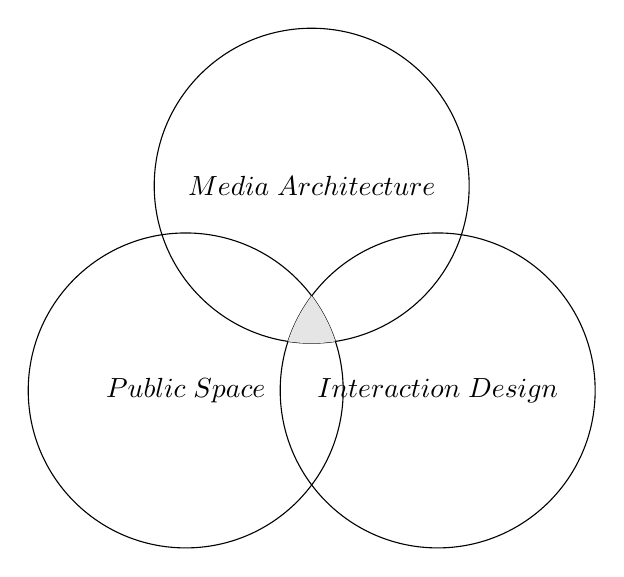
\begin{tikzpicture}
    \draw \firstcircle node {$Media\;Architecture$};
    \draw \secondcircle node {$Interaction\;Design$};
    \draw \thirdcircle node {$Public\;Space$};

    % Now we want to highlight the intersection of the first and the
    % second circle:

    \begin{scope}
      \clip \firstcircle;
      %\fill[red] \secondcircle;
    \end{scope}

    % Next, we want the highlight the intersection of all three circles:

    \begin{scope}
      \clip \firstcircle;
      \clip \secondcircle;
      \definecolor{battleshipgrey}{rgb}{0.9, 0.9, 0.9}
      \fill[battleshipgrey] \thirdcircle;
    \end{scope}

\end{tikzpicture}

\caption[Graphic illustrating key concepts of this PhD]{Urban Interaction Design (urban IxD): The intersection in between the key concepts of \textit{Public Space}, \textit{Interaction Design} in urban space and \textit{Media Architecture} defines the focus of this research. }
\label{keyconcept}
\end{figure}

%%%%%%%%%%%%%%%%%%%%%%%

\subsubsection* {Public Space}

Generally speaking public spaces can be considered as spaces where people come together and perform various activities regardless of their socio-economical status or life style. Public spaces are formed through streets and pavements, parks and plazas and give legal access to every citizen \cite{Lofland_1973}. 

Research into the study of the relationship between architecture, public space and human behaviour has only begun in the 1960s, when journalist and researcher Jane Jacobs came to the conclusion that streets are the very essence of the city \cite{Jacobs_1961}. 
This was based on her observations that liveable streets in small scale neighbourhoods - in contrast to large post war residential structures -  seem to be the places where people meet and where commercial activities animated by amenities such as bars, cafes, restaurants or book stores work successfully. 
%People love watching activities on the sidewalk generated by ordinary people, who run their daily errands. 
%In Jacobs' understanding, this order of movements, what she called the sidewalk ballet, follows a random alignment of improvisation of movements with ongoing new situations which demand human interactions (Jacobs, 1961: 65). Accordingly diversity, density and dynamism are the fundamental columns for a working sidewalk ballet in Jacobs' understanding.

In the 1970s \textit{The Street Life Project} under the leadership of William H. Whyte systematically studied crowding on the streets of New York \label{fig:Whyte}. The research was driven by the question why some public spaces are more popular amongst dwellers than others. The observed imbalance of use in public space suggested practical implications towards a more liveable urban environment\cite{Whyte_1980} \footnote{In addition to the published book about the work conducted by \textit{The Street Live Project} a documentary has been released that clearly demonstrates the applied observations methods: https://vimeo.com/111488563 accessed 25.07.2016}.

%%%%%%%%%%%%%%%%%%%%%%

\begin{figure}[!h] 
\centering
\includegraphics[width=\textwidth]{Illustrations/Whyte_SocialLife.png}
\caption [The Social Life of Public Spaces, 1980] {This screenshot taken from Whyte's documentary \textit{The Social Life of Public Spaces}, 1980, shows the method of observing crowds: A time lapse camera positioned on a raised location facing towards a square with a chronometer in the foreground.}
\label{Whyte}
\end{figure}

%%%%%%%%%%%%%%%%%%%%%%

At the same time, in architectural research a theory called \textit{Space Syntax} generalised that cities need to be considered as an arrangement of architectural layouts that are defined through their relationships between physical space and social life reflected in movement patterns and activities of its inhabitants \cite{Hillier_1989}.
Whilst architects persistently neglected the importance of public spaces for creating social interactions Jan Gehl was one of the pioneers who put his observations and research on public life in cities in practice \cite{Gehl_2013}. 
%Space Syntax aims to analyse the spatial morphology of cities through researching the ‘relation of space to society, [which] is mediated by spatial configuration. Spatial configuration proposes a theory in which we find pattern effects from space to people and from people to space’ \cite{Hillier1998}. A methodological tool-set provided by Space Syntax facilitates the systematic study through spatial analysis and empirical observations of human behaviour such as pedestrian movement or social encounter in the urban realm \cite{AlSayed2013}.

%One of the practitioners is Jan Gehl

%In this context, social encounters can be seen as (un-)planned gatherings amongst strangers or people who know each other. Architectural research has defined ''shared encounters" as mostly context aware, and hence, the type of encounter stage (e.g. bus stop or museum) and its information context impacts the kind of shared encounters. Encounter stages can be defined as public spaces ''on which people negotiate boundaries of a social and cultural nature" \cite{Fatah2009}. For example, at bus stops, social chance encounter happen when people ask for directions or start conversations about the delayed schedule. One objective of the research presented in this paper is to focus on the particular spatial properties, which physical encounter stages require in order to support shared encounters.



%These non-commercial initiatives offer a unique opportunity for exploring novel socio-technological practices in public spaces and provides a promising prospect to regain urban public space as a participatory domain within our cities. Here I see my research in the tradition of researchers such as Jane Jacobs, David Seamon and Jan Gehl who contributed enormously to our present understanding of the social dynamics of public spaces and the prerequisites needed to enable lively cities.  


%Movement is the major component in locational applications. Without movement there is no change in position, therefore there is no data generated from people’s behavior in space.
%Seamon defines movement as ‘any spatial displacement of the body or bodily parts initiated by the person himself or herself’ (Seamon, p.53). He further argues that the body and its extension in space and time are the essential components for an experience. Out of a sequence of movements and gestures evolves the ‘body ballet’ (Seamon, p.54). As soon as we locate the ‘body ballet’ into a specific physical environment we create the ‘place ballet’.
%‘Embodied interaction’ (Dourish, 2001), which describes action of the 'body' or user interacting with embedded technology (and thus potentially linking to social networks) is another important component in location-based applications


%Social encounters are defined as unplanned ad-hoc gatherings amongst (un-) known people. Research has defined ‘shared encounters’ as mostly context aware (e.g. asking a bystander at a bus stop for the next bus to come). Therefore the type of encounter stage (e.g. bus stop) and its information context impacts the kind of shared encounters. Encounter stages are public spaces “on which people negotiate boundaries of a social and cultural nature” (Fatah et al, 2010). An example for a technology-mediated encounter stage is the ‘LED carpet’ project (fig. 1) (Briones et al., 2007)

Only recently digital technologies entered the public domain in form of mobile devices or large electronic surfaces and discussions focus on whether digital technologies affect social interactions in public space have adverse effects \cite{Turkle_2012}, have no impact \cite{Hampton_2015} or can be seen as an opportunity to create mediated participatory experiences \cite{Gordon_2011}. As this discussion only just began theories and knowledge of public space as well as practical applications form the essential basis of this dissertation. Hence the key concept of \textit{Public Space} is followed by a review of research and practice in to Human-Computer Interaction in public space.     
This dissertation is founded on the spirit of Jane Jacobs to look into the small scale interactions in the city and the theories and methodologies developed by \textit{Space Syntax} \cite{AlSayed2013}.

%%%%%%%%%%%%%%%%%%%%%%

\subsubsection* {Interaction Design in Urban Space} 

The discipline of interaction design has evolved from research into Human-Computer Interaction (HCI) and is increasingly concerned with social interactions, which are mediated by computer technologies \cite{Hornecker_2006}. 
Weiser \cite{Weiser_1991} and Dourish \cite{Dourish_2004} predicted a shift in personal computing. Hence, interaction design and technology mediated interactions have moved from home and office desktops onto mobile phones, tablets or public displays into urban spaces \cite{Rogers_2011}. 
Since then, extensive research in HCI has explored social interactions mediated by public displays and put several guides \cite{Muller_2010} and interaction frameworks forward \cite{Vogel_2004}. 
Inevitably, this led to a discussion about space and HCI research has conducted extensive research in understanding technology-mediated human behaviour and social interaction in public space \cite{Fischer_2012, Akpan_2013} \textcolor{red}{(!!!stronger references!!!)}.

In this dissertation I focus on the review of four established frameworks \cite{Brignull_2003, Reeves_2011, Michelis_2011, Fischer_2012} that are considered as important milestones towards an integrated media architectural design space. Each framework describes the relationship between humans and their actions in the presence of large electronic surfaces and in relation to the surrounding space and its physical built environment. 

%%%%%%%%%%%%%%%%%%%%%%

\subsubsection*{Media Architecture}

Since the advent of ubiquitous computing \cite{Weiser_1991}, and its application in urban space in the form of urban computing \cite{Kindberg_2007}, the built environment incorporates architecture and ubiquitous computing technologies.

Seen from an architectural perspective, \textit{Urban Screens} merged into \textit{Media Facades} and became part of the architectural repertoire. Accordingly, \textit{Media Facades} are visually animated architectural surfaces, such as dynamic light facades \cite{Virilio_1991, Fatah_2006, McQuire_2009}.

%%%%%%%%%%%%%%%%%%%%%%

\begin{figure} [h!]
    \centering
        \includegraphics[width=4.5cm]{Illustrations/3.jpg}
        	%\caption[a]{Urban Screen}
      	%\label{UrbanScreen}
        \includegraphics[width=4.5cm]{Illustrations/2.jpeg}
       		%\caption[b]{Media Facade}
       	%\label{MediaFacade}
        \includegraphics[width=4.5cm]{Illustrations/1.jpg}
       		%\caption[c]{Media}
     	%\label{MediaArchitecture}
    \caption[Types of electronic surfaces]{Evolution of large electronic surfaces: Urban Screens (left), Media Facades (centre) and Media Architecture (right).}
    \label{TypesOfSurfaces}
\end{figure}

%%%%%%%%%%%%%%%%%%%%%%

Large electronic surfaces such as \textit{Urban Screens} can be stand-alone or facade-mounted and can be used either temporarily or permanent. 
\textit{Media Facades} incorporate digital media technology already in the building’s surface or are retrofitted to an already existing building. 
Finally \textit{Media Architectures} manifest the idea of embedding media systems already into the initial process of architectural design including architects, designers and media artists. In other words, \textit{Media Architectures} involve multi-dimensional media systems from the very beginning, and electronic surfaces become part of the architectural repertoire.

The notion of architectural facades has always been of informational value, although static. 
%in the way that a facade was considered a social interface connecting the bourgeoisie (private space) with the surrounding city (public space) \cite{Neumeyer_2002}. 
The Gothic cathedrals with their strong sculptural ornaments, sweeping portals and the colourful stained-glass windows transmit a strong visual narrative (Schittich et al., 2006). Martin Pawley (1990) refers to the stained-glass windows as large screens which are powered by natural light.
%Schittich, C., Lang, W. & Krippner, R., 2006. Building skins, Detail Verlag
%Subsection in Schittich: The facade as an information carrier
%Pawley, M., 1990. Theory and design in the second machine age, B. Blackwell.
%Here I could show 2 images: (left) classic facade with ornaments and (right) LED Frieze facade by Christ and Gantenbein (2016)
The advent of Information and Communication Technologies (ICT) has allowed for new types of facades to emerge: information is literally not set in stone anymore \cite{Haeussler_2009}.

Digital information also allows for the anytime exchange of information, such as the flickering advertisement billboards in an inner city, whilst at the same time, the nature of anytime and anywhere information access is changing the relationship between the public and private space (REF). This has led to the development of novel forms of interactions between humans and humans, humans and computers, and humans and architectures. And although Manovich clearly states that the nature of human–computer interactions (HCIs) is interactive per se \cite{Manovich_2001}, architectural surfaces are by far not. 
%Thought needs to be developed

Dalsgaard and Halskov (2010) have outlined the cases and challenges when designing \textit{Media Facades} and suggest considering eight challenges. 
Based on this, a framework for designing complex \textit{Media Facades} has been developed by Halskov and Ebsen (2013), which includes a description of what the difference is between \textit{Media Facades} and conventional displays.
 
To summarise, human-computer interaction and architecture are concerned with the design, implementation and evaluation of digital media technologies and their effect on social interactions in urban spaces. Whilst HCI research in the beginning mostly focused on research in public displays in general, nowadays research differentiates in between \textit{Urban Screens}, \textit{Media Facades} and \textit{Media Architecture}. 
IxD emerged ... 
Yet \textit{Media Architecture} is not an established field, however my aim is to follow key concepts aligned with media architectural research and to eventually contribute to the manifestation of this field. 

%%%%%%%%%%%%%%%%%%%%%%

\section{Research questions}

In this dissertation I consider large electronic surfaces in public spaces, referred to as \textit{Urban Screens}, \textit{Media Facades} or \textit{Media Architecture}, and their potential for mediating social interactions. More specifically I investigate  design aspects and socio-spatial settings in which media architectural installations are embedded. Introducing this research and outlining the key concepts this leads to the central question I address:
%\begin{enumerate}
%  \item [1)]
  
  \textit{How can we design for interactions with large electronic surfaces in public space?}

% \end{enumerate}
 
\noindent Subsequently this question is addressed through the following sub-questions:
  
  \begin{enumerate}
  
  \item  [a)] \textit{Which design aspects need to be considered that enable interactive media architecture?}
 
 \item  [b)] \textit{What kind of novel \textbf{social} practices and behaviours emerge when setting up large electronic surfaces?}
 
 \item  [c)] \textit{How are novel social practices and behaviours around large electronic surfaces related to the properties of public \textbf{spaces}?
(alternatively)What are the spatial conditions large interactive electronic surfaces may afford to evoke interactions in urban spaces?}

\end{enumerate}

%%%%%%%%%%%%%%%%%%%%%%

Little is know so far about the effect digital technologies have on social interactions in urban space. Therefore this research is of exploratory nature and applies a cross-disciplinary methodology.  
The methodological approach has been developed along a practice of \textit{Sentiment Architectures} \footnote{The term and definition of \textit{Sentiment Architectures} comes from the computational advancement to identify people’s emotions in language through \textit{Sentiment Analysis}. We recently published a book with the eponymous title "Sentiment Architectures. A Field Trip to Behaviour and Cognition in Time and Space" \cite{Behrens_2016} } that aims to iteratively design and implement a series of design studies i.e. temporary media architectural installations in public space (coin term: urban prototyping). 
During all studies quantitative and qualitative data has been collected, in one case the period of the data collection can hint towards longitudinal aspects of the implementation of media architectural installations. 
%Two exemplary Sentiment Architectures will explore the role of MAI. The first one called "Smart Citizen Sentiment Dashboard" empowers urban citizen participation by utilizing landmark media facades, while the second one called "Sentiment Cocoon" puts employees’ well-being in the centre of a workplace in London in form of a large interactive installation. In both projects so called media architectural interfaces offer playful interaction modalities delivered through digital technology. Existing Radio Frequency IDentification (RFID) technology and its widespread use in form of ID tags for payless travel purposes or building access, enable participants to engage with the connected surfaces. 
%\textit{Sentiment Architectures} are not a typology. It is a function that derived from a technology called \textit{sentiment analysis} — a tool to identify people’s emotions in language. 
%This idea has been utilised  for an expanded architectural theory and practice. 

%This research began back in 2011, when we first implemented the ubiquitous \textit{I like} button known from social media in physical space. This novel tangible interface that until then existed only in digital space allowed people for the first time to comment on experiences in situ and share them with their remote friends on digital social networks. Back then we were trying to explore this innovative research not only from an academic perspective but also aimed to investigate how we could turn this research and its technology into practice. Since then research and development continued and the idea of situated feedback devices has been further explored. The scope of research was extended towards the urban realm and in particular towards media architecture. During the last three years we have further advanced the idea of tangible feedback interfaces in public spaces. This led to the \textit{Smart Citizen Sentiment Dashboard}, which was produced amongst others for the Viva Cidade festival in Sao Paulo, Brazil (2013), during the Ars Electronica Festival in Linz, Austria (2014) and the European Capital of Culture festivities in Riga, Latvia (2014). The most recent project is the \textit{Sentiment Cocoon} in London, UK (2015 ).


\subsection*{Overview of conducted design studies}

I demonstrate and analyse how temporary media architectural installations might entice people to step out of their daily routines and perceive urban space through a new lens or act differently within it.
This is achieved through a series of design studies, which can be summarised as a field trip into \textit{Sentiment Architectures}. 
The idea of a field trip into \textit{Sentiment Architectures} is an applied research into conscious and shared interfaces in public space that aims to bring together people through giving them the ability to collectively share and project their emotions in public space. The field trip started some time ago with the \textit{Swipe I like} (SIL) project and the \textit{Sentiment Cocoon} is the most advanced prototype so far. In the following I give an overview of the studies carried out and briefly summarise the aims and findings of each study.

%%%%%%%%%%%%%%%%%%%%%%%%%%%%%%%

\begin{table}[h!]
\centering
\resizebox{\textwidth}{!}{
\setlength{\extrarowheight}{8pt}
\begin{tabular}{ccccccc}
\multicolumn{7}{c}{Field trip into Sentiment Architectures} \\ \hline
\multicolumn{2}{c|}{\textit{Pre-Study}} & \multicolumn{3}{c|}{\textit{Study I}} & \multicolumn{2}{c}{\textit{Study II}} \\
\multicolumn{2}{c|}{\textbf{Swipe I like}} & \multicolumn{3}{c|}{\textbf{Smart Citizen Sentiment Dashboard (SCSD)}} & \multicolumn{2}{c}{\textbf{Sentiment Cocoon (SC)}} \\ \hline
\multicolumn{1}{c|}{SIL} & \multicolumn{1}{c|}{VEIV} & \multicolumn{1}{c|}{RIGA} & \multicolumn{1}{c|}{SAOP} & \multicolumn{1}{c|}{LINZ} & \multicolumn{1}{c|}{ARUP} & VIVID \\ \hline
\multicolumn{1}{c|}{\textit{-}} & \multicolumn{1}{c|}{\textit{DIY display}} & \multicolumn{1}{c|}{\textit{Urban Screen}} & \multicolumn{1}{c|}{\textit{Media Facade}} & \multicolumn{1}{c|}{\textit{Media Architecture}} & \multicolumn{1}{c|}{\textit{Media Architecture}} & \textit{Media Architecture}
\end{tabular}
}
\caption[Overview of conducted design studies]{Overview of conducted design studies including the types of electronic surfaces.}
\label{study_overview}
\end{table}


%%%%%%%%%%%%%%%%%%%%%%%%%%%%%%%

\begin{singlespace}{

\begin{labeling}{projects}

\item [\textbf{SIL}] 
\begin {itemize} 
\footnotesize
\item [\textit{aims}] Enhancing the engagement of museums visitors with exhibition content through implementing situated and shared digital technologies in public space. 
\item [\textit{objectives}] Designing and implementing a novel tangible interface (i.e. physical \textit{I like} button) in a museum space that lets people share their views about exhibition content with their digital networks. \newline Observing visitors' practices and behaviours when engaging with museum content through the interactive system. 
\item [\textit{findings}] Such systems can enhance engagement and reveal emergent social behaviours. \newline Lack of a immediate feedback in form of a display.

\end{itemize}

\item [\textbf{VEIV}] 
\begin {itemize}
\footnotesize
\item [\textit{aims}] Providing immediate visual feedback to participants engaging with novel tangible interfaces.
\item [{objectives}] Connecting physical {I like} button to a large electronic surface (i.e. {DIY display} )in public space to provide users with immediate visual feedback.
\item [\textit{findings}]  Positioning of the DIY surface determines interactions and structures the surrounding space. \newline Identifying the importance of the ambient character of large electronic surfaces.
\end{itemize}

\item [\textbf{RIGA}] 
\begin {itemize}
\footnotesize
\item [\textit{aims}] Exploring the effect of the positioning of large electrinic surfaces on the existing flow of people in urban space.
\item [{objectives}] Design iteration of tangible interface (i.e. {Sentiment Dashboard}) and careful positioning of the {Sentiment Dashboard} and the attached electronic surface (i.e. {Urban Screen}) in urban space.
\item [\textit{findings}] Novel media architectural interfaces in public space can disrupt flows of people and provoke emergent behaviours, which ultimately change the dynamics of a physical space.
\end{itemize}

\item [\textbf{SAOP}]
\begin {itemize}
\footnotesize
\item [\textit{aims}] Exploring up to what scale the designed interactive system works in terms of human behaviour and social interactions.
\item [\textit{objectives}] Connecting the the \textit{Sentiment Dashboard} to a large existing \textit{Media Facade}. 
\item [\textit{findings}] Positioning and size of tangible interfaces relates to size of \textit{Media Facades}. \newline Confirming the importance of ambient perception of media architectural installations. \newline Interactions with \textit{Media Facades} and the visual feedback on the electronic surface alter the appearance of a building.
\end{itemize}
 
\item [\textbf{LINZ}] 
\begin {itemize}
\footnotesize
\item [\textit{aims}] Exploring the ambient character of large electronic displays and the appearance of Media Architecture during day and night and its effect on human behaviours and social interactions.  
\item [\textit{objectives}]Connecting the the \textit{Sentiment Dashboard} to a large existing three dimensional \textit{Media Architecture}.
\item [\textit{findings}] Resolution of electronic surface and shape impact the visual feedback displayed. \newline Interactions with \textit{Media Architectures} and the visual feedback displayed on the electronic surface alter the appearance of a building.
\end{itemize}

\item [\textbf{ARUP}]
\begin {itemize}
\footnotesize
\item [\textit{aims}] Designing and implementing of temporary \textit{Media Architecture} based on the findings from previous studies.  \newline Incorporating the process of fabrication in public to explore social interactions. \newline Exploring the longitudinal effects on interactions of media architectural systems.
\item [\textit{objectives}] Collaborating with a large team of engineers and designers to implement our design of a self fabricated \textit{Media Architecture}.
\item [\textit{findings}] Only the appearance of a novel large electronic surface attracts people and triggers social interactions. \newline Bringing the process of fabrication into the public creates social interactions \newline Decrease of interactions after a couple of weeks.
\end{itemize}

\item [\textbf{VIVID}] 
\begin {itemize}
\footnotesize
\item [\textit{aims}] Designing and implementing a different temporary \textit{Media Architecture} with a novel tangible interface in a public outdoor space to confirm our previous findings.
\item [{objectives}] Designing and implementing a more intuitive tangible interface (i.e.{Palm Pulse Reader}).  
\item [\textit{findings}] Different tangible interface to confirm findings regarding the emergence of novel behaviours and social interactions. 
\end{itemize}

\end{labeling}
}
  
  \end{singlespace}


\section{Chapter outline summary}

This dissertation consists of seven chapters. The first introductory chapter provides an overview of the motivation, key concepts and the research questions. The background chapter summarises related works concerned with the key concepts of Media Architecture, Public Space and Urban HCI. Existing interaction frameworks that have explored the role of awareness, actor, action, and physical space will be juxtaposed to clarify triangular relation between the key concepts. Based on this evaluation I will introduce our notion of \textit{Media Architectural Interfaces} (MAIs). Running up to the case study in chapter five I will layout my research-through-design based methodology. The case study chapter is summarised as \textit{Field trip into Sentiment Architectures} and starts with two pre-studies before actually processing the two main studies namely \textit{Smart Citizen Sentiment Dashboard} and \textit{Sentiment Cocoon}. Chapter 6 discusses the findings of the studies and categorises interactive media architecture in the light of the MAI framework. Finally this dissertation concludes with an outlook for future work in this field.  

%As a starting point I review existing implementations and research in the field of media architecture and human-computer interaction in urban space and focus on four established frameworks that we consider as important milestones towards an integrated media architectural design space. Each framework describes the relationship between humans and their actions in the presence of programmable electronic displays and in relation to the surrounding space and its physical built environment. 

%Based on this review, I will introduce the notion of Media Architectural Interfaces (MAI) in order to clarify the relation between large electronic surfaces, attached interfaces within the given context to structure these new practices.  
%MAI describe an ecology of tangible and non-tangible interfaces. 
%They can be considered as interactive systems in public spaces, which potentially entice people to step out of their habitual routine and perceive their surrounding through a new lens or act differently within it. 
%In more detail, MAI are a syndissertation of situated and shared interfaces. 
%They mediate participants' engagement with large programmable surfaces such as \textit{Urban Screens}, \textit{Media Facades} or \textit{Media Architecture}.   
%MAIs confront us with novel types of interactions between humans and technology in public space. They create platforms for social interactions which are mediated by interactive systems. New spatial practices emerge.
%To illustrate this framework I categorise a selection of temporary media architectural installations, which I consider best practice.

%In a series of installations which I have conducted I will demonstrate ...

%Finally, I discuss the multi-layered interaction frameworks with regard to the conducted design studies and summarise the relevant communality of these design studies in a taxonomy. The aim of this categorisation is to provide design implications for future MAI projects. Ultimately, this may support the design and development of novel and sustainable interactive systems in the domains of urban screens, media facades, and media architecture.

%This dissertation aims to contribute to the growing field of \textit{Media Architecture}. 


\section{Contribution}

This dissertation contributes empirically to research and practice in the emerging field of \textit{Media Architecture}. Through a theoretical review of existing works at the intersection between the fields of \textit{Public Space}, \textit{Human-Computer Interaction} and \textit{Media Facades} and design based through a series of studies I further advance knowledge to the understanding of technology mediated interactions in public space an the role of media architecture within. Hereby this research adds value to cross-disciplinary collaborations  between design, technology and research.

\subsubsection*{Theoretical contribution}
This dissertation summarises the state of the art in \textit{Public Space} research, \textit{Human-Computer Interaction} research and large electronic surfaces such as \textit{Urban Screens}, \textit{Media Facades} and \textit{Media Architecture} to assist in the manifestation of the field of \textit{Media Architecture}.
Part of this investigation is the categorisation of various forms of large electronic displays, the plotting of existing spatial interaction frameworks against each other and eventually the introduction of a framework for \textit{Media Architectural Interfaces} (MAI). 
A cross-disciplinary practice-based methodology has been developed to support future research in the field of temporary media architectural installations. 

\subsubsection*{Design contribution}
Through the series of case studies I describe the design process and eventually contribute to knowledge through identifying challenges and implications when designing for interactions with media architectural installations in public space. 
At the same time I contribute to the research in HCI either through confirming or  discovering emergent behaviours around technology mediated installations.
Eventually this may guide architects, urban designers, interaction designers, curators and artists to consciously use media architectural installations to enrich public spaces.
Whilst at the same time I provide insights into the challenges and opportunities of cross-disciplinary design teams in the field of media architecture.

